\documentclass[t,slidestop,compress,mathserif,color=option,hyperref={pdfstartview={Fit},pdfpagelayout={SinglePage},pdfpagemode={UseOutlines}}]{beamer}

%\usepackage[envcountsect]{beamerarticle}

\usepackage{general-beamer}

\usetheme{Madrid}
\usecolortheme{seahorse}

%\usepackage{beamercolorthemeCalPoly}
%\usepackage{beamerinnerthemeCalPoly}
%\usepackage{beamerouterthemeCalPoly}
%\usepackage{beamerthemeCalPoly}

\usepackage{tikz}

\hypersetup{
  pdfstartview={Fit}
  pdfpagelayout={SinglePage}
  pdfpagemode={UseOutlines}
}

\xdefinecolor{blue}{rgb}{0.0,0.2,0.8}
\newcommand{\blue}[1]{{\color{blue}#1}}
\newcommand{\emblue}[1]{\emph{\color{blue}#1}}
\xdefinecolor{purple}{rgb}{0.4,0.0,0.6}
\newcommand{\purple}[1]{{\color{purple}#1}}
\xdefinecolor{red}{rgb}{0.8,0,0.2}
\newcommand{\red}[1]{{\color{red}#1}}
\xdefinecolor{green}{rgb}{0.2,0.6,0.2}
\newcommand{\green}[1]{{\color{green}#1}}
\newcommand{\CPgreen}[1]{{\color{CPgreen}#1}}

\newcommand*\diff{\mathop{}\!\mathrm{d}} % command for differential operator
\newcommand{\integral}[4][x]{\ensuremath{\displaystyle \int_{#3}^{#4} #2 \diff #1}}
    
\begin{document}

\allowdisplaybreaks

\title[Quaternions]
    {2D Number Systems in the Quaternions 
        \begin{align*}
            \left\{t+xi+yj+zk: 
            \begin{aligned}
                & t, x, y, z \in \bR, \\
                & i^2 = j^2 = -1, \\
                & ij = -ji = k 
            \end{aligned}
            \right\}
        \end{align*}     
    }
\author[Andy, Ian, Bailey]
    {Andy Haase, Ian Gallagher, Bailey Wickham \\ Dr. Brussel}

\begin{frame}
  \titlepage
\end{frame}

\begin{frame}{Introduction}
    \begin{itemize}
        \item We are familiar with $\bR^1$ (line), $\bR^2$ (plane), $\bR^3$ (space) in everyday life. We are studying $\bR^4$ with additional structure.  
        \item We are studying the quaternions (\bH), a 4D number system with a geometric interpretation.
        \item Of particular interest is the structure of the planes inside of $\bR^4$.
        \item Q. Is there a way to "see" all of the planes at once? \\
              A. The representation of these planes as points on another geometric object forms what is called a \textit{moduli space}.  
       \item Example: Take all directed lines through the origin in $\bR^2$. They can be represented as the points of a circle around the origin. This circle is a picture of \textbf{all} directed lines on the plane
    \end{itemize}
    \centering
    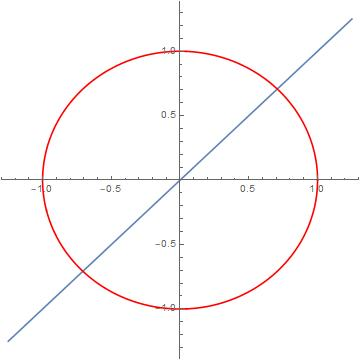
\includegraphics[scale=.15]{H Pres - 8-20-20/CircleModuliSpace.jpg}
    \end{frame}

\subsection{Structure}

\begin{frame}{A Number System in 4 Dimensions}
  \begin{itemize}
      \item We all know how to define an addition on a set of points on a plane. We simply add, term-wise.
      \item For example (1,2)+(3,4)=(4,6) (Vector addition).
      \item But can we define a multiplication on the plane?
      \item We could multiply term-wise as well and we call this \bR x \bR
      \item Another way to define a multiplication on a plane is \bC.
      \item This means the plane is a "number system."
      \item Q. Can we make 4 space into a "number system"? \\
            A. YES! There are 2: \bH and $M_2(\mathbb{R})$.
      \item These "number system" constructions are called Central Simple Algebras (CSA's)
  \end{itemize}
 \end{frame}
 
 \begin{frame}{Planes Through the Real Axis}
  \begin{itemize}
      \item Interestingly, both of these constructions (\bH and $M_2(\mathbb{R})$) in 4 dimensions, unlike our construction of \bC on the plane, have \textit{non-commutative} multiplications. i.e. $ab\ne ba$
      \item Our research pertains to the different planes inside of these 4 dimensional spaces which become number systems under the induced multiplication. 
      \item This forces them to contain the real line. 
      \item The induced multiplication on these planes is \textit{commutative}.
      \item In fact, these are the maximal commutative sub-algebras of \bH and $M_2(\mathbb{R})$
      \item Our goal is to find a moduli space for these planes.
  \end{itemize}
\end{frame}

\begin{frame}{The Sphere of Planes in 4 Dimensions}
    \begin{itemize}
        \item The planes that include the $x$-axis in 3D space form a "circle of planes".This is a moduli space for these planes.
        \item We found that in $\mathbb{R}^4$ the planes that include the $t$-axis form a "\textit{sphere} of planes".
        \item Therefore the sphere is a moduli space representing these "number system" planes.
        \item In \bH, we found that these planes are all complex planes. But over $M_2(\mathbb{R})$ we found that there are actually 3 different "types" of planes.
    \end{itemize}
    \begin{align*}
            \bH = \left\{t + xi + yj + zk : t, x, y, z \in \bR, i^2=j^2=ijk=-1 \right\}
    \end{align*}
\end{frame}
\begin{frame}{2D Number Systems in \bH}
    \begin{itemize}
        \item The group $S^3$ acts transitively on these complex planes through a group action called \textit{conjugation} on each plane element. Therefore, $S^3$ acts transitively on $S^2$. 
        \item The stabilizer of a point is a circle. 
    \end{itemize}
    
    \begin{figure}
        \centering
        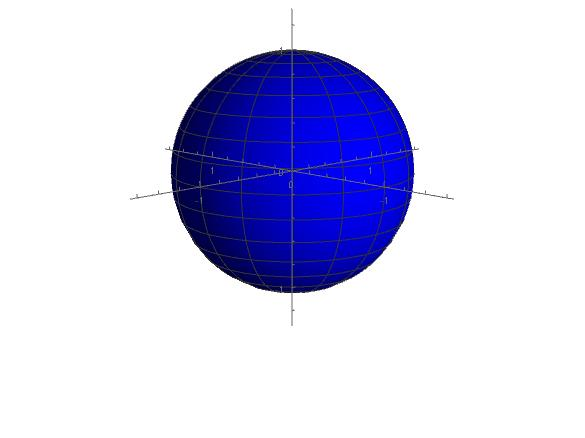
\includegraphics[trim = 0 120 0 0, scale=.4]{H Pres - 8-20-20/QuatSphere.jpg}
        \caption{Planes in $\bH$}
        \label{fig:H}
    \end{figure}
\end{frame}

\begin{frame}{2D Number Systems in $M_2(\bR)$}
\begin{itemize}
    \item We found that there exist complex planes inside of $M_2(\bR)$, but unlike in \bH, there are other 2D number systems with different multiplications contained.
    \item The types are \bC, $\bR \times \bR$, and a 'degenerate' case, we call a {\it nilpotent plane}.
    \item An analog to $S^3$ acts on each set of planes in $M_2(\bR)$
\end{itemize}

\begin{minipage}{.45\textwidth}
\begin{figure}
    \centering
    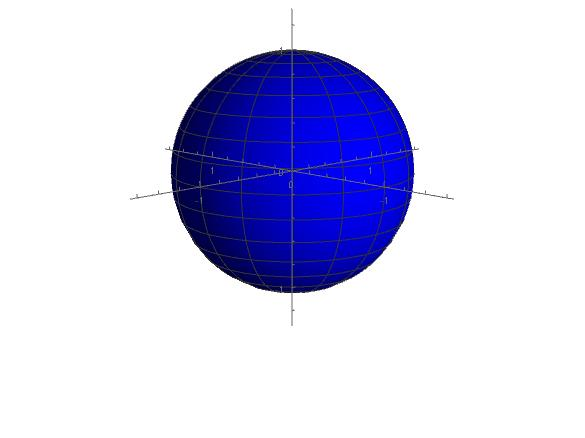
\includegraphics[trim = 0 120 0 0, scale=.25]{H Pres - 8-20-20/QuatSphere.jpg}
    \caption{Planes in $\bH$}
    \label{fig:H}
\end{figure}
\end{minipage}
\begin{minipage}{.45\textwidth}
\begin{figure}
    \centering
    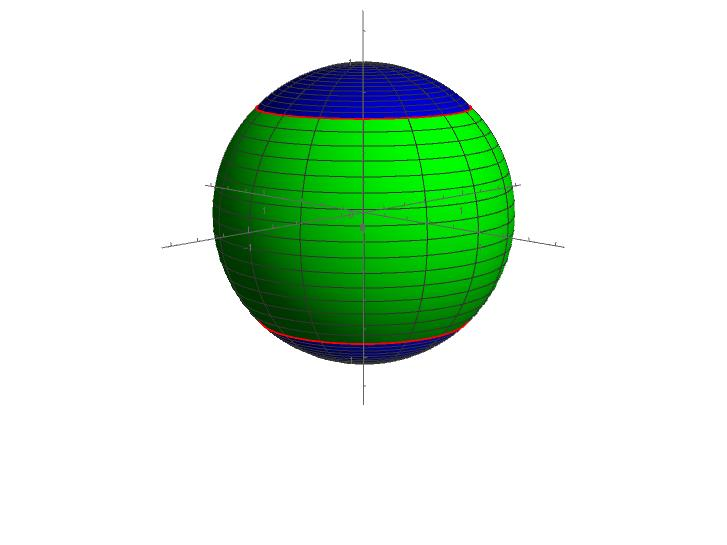
\includegraphics[trim = 0 150 0 0, scale=.2]{H Pres - 8-20-20/MatricesSphere.jpg}
    \caption{Planes in $M_2(\bR)$}
    \label{fig:my_label}
\end{figure}
\end{minipage}    

\end{frame}

%\begin{frame}{Conjugacy classes of \bC in \bH}
%    \begin{itemize}
%        \item We have a space of embeddings of \bC into \bH, but how are these planes related? 
%        \item It turns out all the complex planes in \bH are conjugate. Conjugate elements are "closely related".
%        \item Similar matrices are an example of a conjugate elements.
%        \item Remember, similar matrices are actually the same under a change of basis. This is actually \textit{exactly} what we are doing. These "similar" planes are the same under relabeling.
%        \item All complex planes are conjugate in \bH, there is only one conjugacy class
%        \item Another way to say this is that the group action has a single orbit
%    \end{itemize}
%\end{frame}

\begin{frame}{Generalized Quaternions} 
\begin{itemize}
    \item The construction of the quaternions can be generalized, let $\mathbb{F}$ be a field:
    \begin{block}{Generalized Quaternions}
    \begin{center}
    $A_{a,b}(\mathbb{F}) = \{t + bi + cj + dk : t,b,c,d \in \mathbb{F}\} \\
    \text{ where }i^2 =a, j^2 = b, \text{ and } ij = -ji=k $
    \end{center}
    \end{block}
    \item The quaternions we considered previously are $\bH=A_{-1,-1}(\bR)$
    \item As described above, \bH is a Central Simple Algebra (CSA), we are interested in classifying other CSAs over \bR. Our choice of $a,b$ in $A_{a,b}(\bR)$ determine the CSAs we get.
    \item Over \bR, there are two CSAs, the 2x2 matrices $(M_2(\bR))$, and \bH
\end{itemize}
\end{frame}
\end{document}